%% SANER 2027 -- Short Papers and Posters (SP&P) Track
%% Limit: SIX pages INCLUDING all text, figures, references and appendices.
%%        There is no separate reference allowance on this track.
%% Format: IEEE Conference Proceedings Formatting Guidelines; title 24pt,
%%        text 10pt; LaTeX must use \documentclass[10pt,conference]{IEEEtran}.
%% Formatting per SANER guidance: IEEEtran, 10pt, conference option, and
%%        WITHOUT the compsoc or compsocconf option.
%% Double-anonymous: author names and affiliations omitted; references to the
%%        authors' own prior work in the third person.
\documentclass[10pt,conference]{IEEEtran}
\IEEEoverridecommandlockouts

\usepackage{cite}
\usepackage{amsmath,amssymb}
\usepackage{booktabs}
\usepackage{xcolor}
\usepackage{tikz}
\usepackage[hidelinks]{hyperref}

\newcommand{\killk}[1]{Kill@#1}
\definecolor{oaccent}{HTML}{2F5D8C}
\definecolor{orule}{HTML}{B9C2CE}

\begin{document}

\title{A Development Gain That Did Not Survive Locking\\
in LLM-Based Mutation Test Generation}

\author{\IEEEauthorblockN{}\IEEEauthorblockA{}}

\maketitle

\begin{abstract}
Supervised fine-tuning of a 1.5B-parameter code model for mutation test
generation raised \killk{8} from $0.605166$ to $0.695572$ on the panel used to
select its checkpoints. On a locked split not used to select a checkpoint, tune
a prompt, or set a threshold, the same checkpoint gave $+3.4346$ percentage points ($450/757 \to 476/757$) with an
exact two-sided McNemar $p = 0.0783$ against a threshold of $p < 0.01$ fixed
before either arm ran; the untrained base model was retained. Over that same
comparison, the fraction of candidates passing against the \emph{correct}
implementation fell by $11.8726$ points while parse and execution validity did
not regress. We report both as negative and inconclusive evidence, and we are
explicit that a non-significant difference is not evidence of no difference. We
also report that executing the complete measurement path at full scale on a
permitted split reproduced a prior \killk{8} of $0.605166$ exactly --- evidence
of execution fidelity, not of model quality.
\end{abstract}

\begin{IEEEkeywords}
mutation testing, LLM test generation, negative results, evaluation integrity
\end{IEEEkeywords}

\section{Introduction}

Mutation kill rate is an attractive score for LLM-generated tests: objective,
executable, independent of coverage heuristics. But \killk{k} alone can be
misleading when candidate and reference validity are not reported alongside it.
A test that fails against every implementation still distinguishes a mutant from
its reference, so a kill-rate-only evaluation cannot separate a discriminating
test from a broken one.

This short paper reports three findings from one controlled study, chosen
because each is defensible on its own evidence.

\begin{enumerate}
  \item A selection-panel gain of $9.04$ \killk{8} points corresponded to
        $+3.4346$ points on a locked split --- and the locked result did not
        meet a predeclared significance threshold.
  \item Candidate \emph{reference} validity regressed by $11.8726$ points over
        the same locked comparison, while parse and execution validity did not.
  \item Running the full measurement path at full scale on a permitted split
        reproduced a previously recorded value exactly, which is what makes the
        pipeline's other numbers interpretable.
\end{enumerate}

\section{Setting}

The generator is \texttt{Qwen2.5-Coder-1.5B-Instruct} at a pinned immutable
revision. All measurements run under one protocol, frozen and identified by
digest before use: eight candidates per target, temperature $0.7$, top-$p$
$0.9$, seed $42$, whole-output candidate parsing, raw-output retention, a 1024
token completion limit, no reranking, no feedback rounds.

Two panels matter. The \emph{development} panel ($n = 542$ function targets)
selected the checkpoints it scores, so its figures are selection statistics and
not generalization estimates. The \emph{locked} split ($n = 757$) was not used
to select a checkpoint, tune a prompt, or set a threshold; it determined the
predeclared promotion decision and was read once. Before either locked arm ran, a promotion rule was
committed to a hash-bound receipt requiring all of: \killk{8} gain
$\geq +3.0$ points, net gain $\geq 15$ functions, and exact two-sided McNemar
$p < 0.01$.

A fourth split was reserved for a single final measurement. It was consumed by
an authorized attempt that produced \textbf{zero candidates and zero metrics},
and may never be rerun. No number in this paper derives from it.

\section{Results}

\begin{table}[t]
\caption{\killk{8} by panel. The two blocks are not comparable quantities: the
development panel chose the checkpoints it scores.}
\label{tab:main}
\centering
\footnotesize
\begin{tabular}{@{}llrrr@{}}
\toprule
Panel & Arm & \killk{8} & Fns & Wilson 95\% \\
\midrule
\multicolumn{5}{@{}l}{\textit{Development --- selection-only, $n = 542$}}\\
& base  & 0.605166 & 328 & [0.5634, 0.6454] \\
& A@431 & 0.695572 & 377 & [0.6556, 0.7328] \\
\midrule
\multicolumn{5}{@{}l}{\textit{Locked validation --- $n = 757$}}\\
& base  & 0.594452 & 450 & [0.5591, 0.6289] \\
& A@431 & 0.628798 & 476 & [0.5938, 0.6625] \\
\midrule
\multicolumn{5}{@{}l}{\textit{Paired locked difference}}\\
& gained / lost / net & \multicolumn{3}{r}{$+114$ / $-88$ / $+26$} \\
& \killk{8} delta & \multicolumn{3}{r}{$+3.4346$ points} \\
& McNemar exact $p$ & \multicolumn{3}{r}{$0.0783$} \\
& requirement (predeclared) & \multicolumn{3}{r}{$p < 0.01$ --- \textbf{not met}} \\
& decision & \multicolumn{3}{r}{\textbf{retain base model}} \\
\bottomrule
\end{tabular}
\end{table}

\subsection{Development overstated the locked result}

Table~\ref{tab:main} and Fig.~\ref{fig:cmp} give the comparison. The selection
panel showed $+9.04$ points; the locked split showed $+3.4346$, roughly
$2.6\times$ smaller. This is what selection bias predicts when a panel chooses
the checkpoint it then scores.

The locked point estimate is \emph{positive}. With 202 discordant pairs
($114$ versus $88$), an exact two-sided McNemar test \cite{mcnemar1947note}
gives $p = 0.0783$ against a required $p < 0.01$, so the predeclared criterion
failed and the base model was retained. We stress the reading: the data are
insufficient to conclude an effect at the standard set in advance. That is
\textbf{not} a finding of no effect \cite{wasserstein2016asa,amrhein2019retire},
and the question cannot now be settled on this split, which has been used to
decide.

\begin{figure}[t]
\centering
% x = (Kill@8 - 0.54) * 22 cm. Values verbatim from the result receipts.
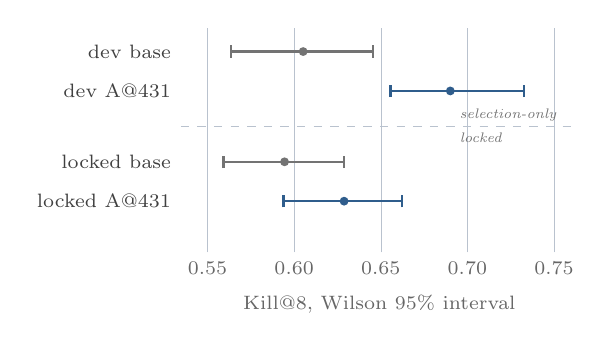
\begin{tikzpicture}[font=\scriptsize,x=1cm,y=1cm]
  \foreach \v/\lx in {0.55/0.22, 0.60/1.32, 0.65/2.42, 0.70/3.52, 0.75/4.62}{
    \draw[orule,very thin] (\lx,-0.3) -- (\lx,2.55);
    \node[below,text=black!60] at (\lx,-0.3) {\v};
  }
  \foreach \y/\lab/\lo/\pt/\hi/\c in {%
    2.25/{dev base}/0.515/1.434/2.320/black!55,
    1.75/{dev A@431}/2.542/3.303/4.242/oaccent,
    0.85/{locked base}/0.420/1.198/1.955/black!55,
    0.35/{locked A@431}/1.184/1.954/2.687/oaccent}{
      \draw[\c,line width=0.9pt] (\lo,\y) -- (\hi,\y);
      \draw[\c,line width=0.9pt] (\lo,\y-0.08) -- (\lo,\y+0.08);
      \draw[\c,line width=0.9pt] (\hi,\y-0.08) -- (\hi,\y+0.08);
      \fill[\c] (\pt,\y) circle (1.6pt);
      \node[left,text=black!75] at (-0.12,\y) {\lab};
  }
  \draw[orule,dashed] (-0.12,1.30) -- (4.9,1.30);
  \node[right,text=black!55,font=\tiny] at (3.3,1.44) {\textit{selection-only}};
  \node[right,text=black!55,font=\tiny] at (3.3,1.16) {\textit{locked}};
  \node[below,text=black!60] at (2.4,-0.72) {\killk{8}, Wilson 95\% interval};
\end{tikzpicture}
\caption{The locked pair (lower rows) is positive but not significant under the
predeclared rule; its intervals overlap. Development and locked rows measure
different populations and must not be subtracted.}
\label{fig:cmp}
\end{figure}

\subsection{Reference validity regressed}

Over the same locked comparison, the fraction of candidates that pass against
the \emph{correct} implementation fell from $0.452114$ to $0.333388$ --- a
$-11.8726$ point change --- and targets with any reference-valid candidate fell
from $675$ to $566$. Parse validity rose $0.1486$ points and execution validity
rose $1.3870$ points over the same comparison, so this is not general
degradation: the tuned model emits \emph{more} usable tests that are
\emph{more often} wrong about the reference. The direction held in all four
development arms, making it a property of this supervision family rather than of
one checkpoint.

A kill-rate-only report would not show this, and it moves opposite to the
headline. A tool selected on kill rate alone may be selected against test
quality.

\subsection{The pipeline computes what it claims}

Executing the complete path --- receipt verification, admission, mode-aware
scoping, generation, whole-output parsing, safe execution, raw-output retention,
progress writing and scoring --- at full scale on the permitted panel produced
$4{,}336$ candidates over $542$ targets with $4{,}336$ retained raw outputs,
$4{,}336$ digests, zero missing and zero mismatched, and zero mismatches on an
independent recomputation. Its \killk{8} was $0.605166$: identical to the value
previously recorded for the same model on the same panel under the same
evaluation-scope digest. No weights were written and no adapter was loaded.

This is evidence of \emph{execution fidelity}. It is not a model-performance
result, not a generalization estimate, not a selection result, and not a
substitute for the final measurement that was lost.

That measurement was lost to a narrow defect worth naming, because it is cheap
to avoid: the final-run path applied a record-admission rule to \emph{every}
record before the scope filter that the established evaluator had always applied
first, and so refused records the pipeline was always going to exclude. The
component was unreachable until the one-time authorization was spent, and had
therefore never been executed against real data. Running the same selector
against permitted splits reproduces the rejection immediately, at no cost.

\section{Claim Status}

\begin{table}[t]
\caption{What this study does and does not support.}
\label{tab:claims}
\centering
\footnotesize
\begin{tabular}{@{}p{0.94\columnwidth}@{}}
\toprule
\textbf{Established} \\
\midrule
Selection-panel \killk{8} $0.605166 \to 0.695572$; locked
$0.594452 \to 0.628798$ for the same checkpoint. \\
Paired locked difference $+3.4346$ points, $+114/-88$, net $+26$, exact
McNemar $p = 0.0783$; predeclared $p < 0.01$ not met; base retained. \\
Reference validity fell $11.8726$ points; parse and execution validity did not
regress. \\
A full-scale permitted-split rehearsal reproduced a prior \killk{8} of
$0.605166$ exactly, with complete raw-output integrity and no weights written. \\
\midrule
\textbf{Inconclusive} \\
\midrule
Whether fine-tuning improves \killk{8} on unseen data: undetermined at this
sample size. Positive point estimate, threshold not met, \emph{not} evidence of
no effect. \\
Whether the validity regression is intrinsic to the objective or specific to
this recipe. \\
\midrule
\textbf{Unavailable} \\
\midrule
No final-test result exists for any arm. \\
No native repository-level kill rate exists; records of that mode are excluded
from every rate reported. \\
No comparison against any external baseline tool exists; none was bundled or
executed in any measurement reported here. \\
\bottomrule
\end{tabular}
\end{table}

\section{Threats to Validity}

\emph{Construct.} \killk{k} credits any distinguishing candidate including a
universally failing test, which is why reference validity is reported beside it;
mutants are an imperfect proxy for real faults
\cite{just2014mutants,papadakis2018mutationscores}.
\emph{Internal.} One locked criterion failed through a defect of ours --- an
adapter-specific digest placed inside a contract required to be identical across
arms --- recorded as a failure, not reinterpreted; the decision does not rest on
it, as the significance criterion failed independently.
\emph{External.} One model, one corpus, one supervision family, one seed; no
claim that the ratio or trade-off transfers.
\emph{Statistical.} A single paired exact test on 202 discordant pairs, reported
with Wilson intervals \cite{wilson1927probable,arcuri2014hitchhiker}, without
converting non-significance into a null result.

\section{Conclusion}

An apparent development gain did not establish reliable improvement on a locked
split, and candidate reference validity regressed substantially over the same
comparison while parse and execution validity did not. Report a validity metric
beside the kill rate; freeze the decision rule before the run; and execute the
whole measurement path on permitted data at full scale before anything
irreversible depends on it.

\section*{Data Availability}

An anonymized replication package accompanies this submission. It contains the
frozen generation protocol and its digest, the promotion rule as committed
before the locked run, the development and locked result receipts, the rehearsal
receipt and its sanitised execution receipt, and per-figure data files each
carrying the SHA-256 of its source receipt. Every number in this paper is
traceable to one of those receipts.

Raw generated model outputs are retained but excluded from the package because of
their volume; their digests are published so any retained output can be verified
without redistribution. No material from the consumed split is included, and none
exists. The package is hosted on an anonymous-capable archive and contains no
repository host, account or link that could identify the authors.

\bibliographystyle{IEEEtran}
\bibliography{references}

\end{document}
